\documentclass[11pt]{book}
\usepackage{palatino}
\usepackage{amsfonts,amsmath,amssymb}
% \usepackage{graphicx}


\ifx\pdftexversion\undefined
    \usepackage[dvips]{graphicx}
\else
    \usepackage[pdftex]{graphicx}
    \usepackage{epstopdf}
    \epstopdfsetup{suffix=}
\fi


\begin{document}

%%%%%%%%%%%%%%%%%%%%%%%%%%%%%%%%%%%%%%%%
% Problem Set 3
%%%%%%%%%%%%%%%%%%%%%%%%%%%%%%%%%%%%%%%%

\pagestyle{empty}
{\noindent\bf Spring 2023 \hfill Firstname M.~Lastname}
\vskip 16pt
\centerline{\bf University of Central Florida}
\centerline{\bf College of Business}
\vskip 16pt
\centerline{\bf QMB 6911}
\centerline{\bf Capstone Project in Business Analytics}
\vskip 10pt
\centerline{\bf Solutions:  Problem Set \#2}
\vskip 32pt
\noindent
%
\section*{Data Description}
% 
By engaging an industry consultant to gather relevant and appropriate 
information, your firm has been able to put together data concerning 248 
different fly-fishing reels, over one-half of which are produced in the 
United States, with the remainder being produced in Asia---either in China 
or Korea.  These data are contained in the file {\tt FlyReels.csv}, which is
available in the {\tt Data} folder.
Each fly-fishing reel in the data set is a row, while the columns correspond 
to the variables whose names and definitions are the following:
\bigskip
\begin{table}[ht]
\centering
\begin{tabular}{ll}
  \hline
    Variable & Definition \\
  \hline

    {\tt Name}        &product name (a string) \\ 
    {\tt Brand}       &brand name (a string) \\ 
    {\tt Weight}      &weight of reel in ounces (a real number) \\ 
    {\tt Diameter}    &diameter of reel in inches (a real number) \\ 
    {\tt Width}       &width of reel in inches (a real number) \\ 
    {\tt Price}       &price of reel in dollars (a real number) \\ 
    {\tt Sealed}      &whether the reel is sealed; {\tt "Yes"} versus
                        {\tt "No"} (a string) \\ 
    {\tt Country}     &country of manufacture, (a string) \\ 
    {\tt Machined}    &whether the reel is machined versus cast;
                        machined={\tt "Yes"}, \\ 
                      &while cast={\tt "No"} (a string) \\ 
  \hline
\end{tabular}
%\caption{Summary of Numeric Variables}
%\label{tab:summary}
\end{table}


\section*{Empirical Distribution Function of Fly Reel Prices}

Figure \ref{fig:ecdf_prices} is 
a plot of the empirical cumulative distribution function (CDF) of fly reel prices. 


\begin{figure}[h!]
  \centering
  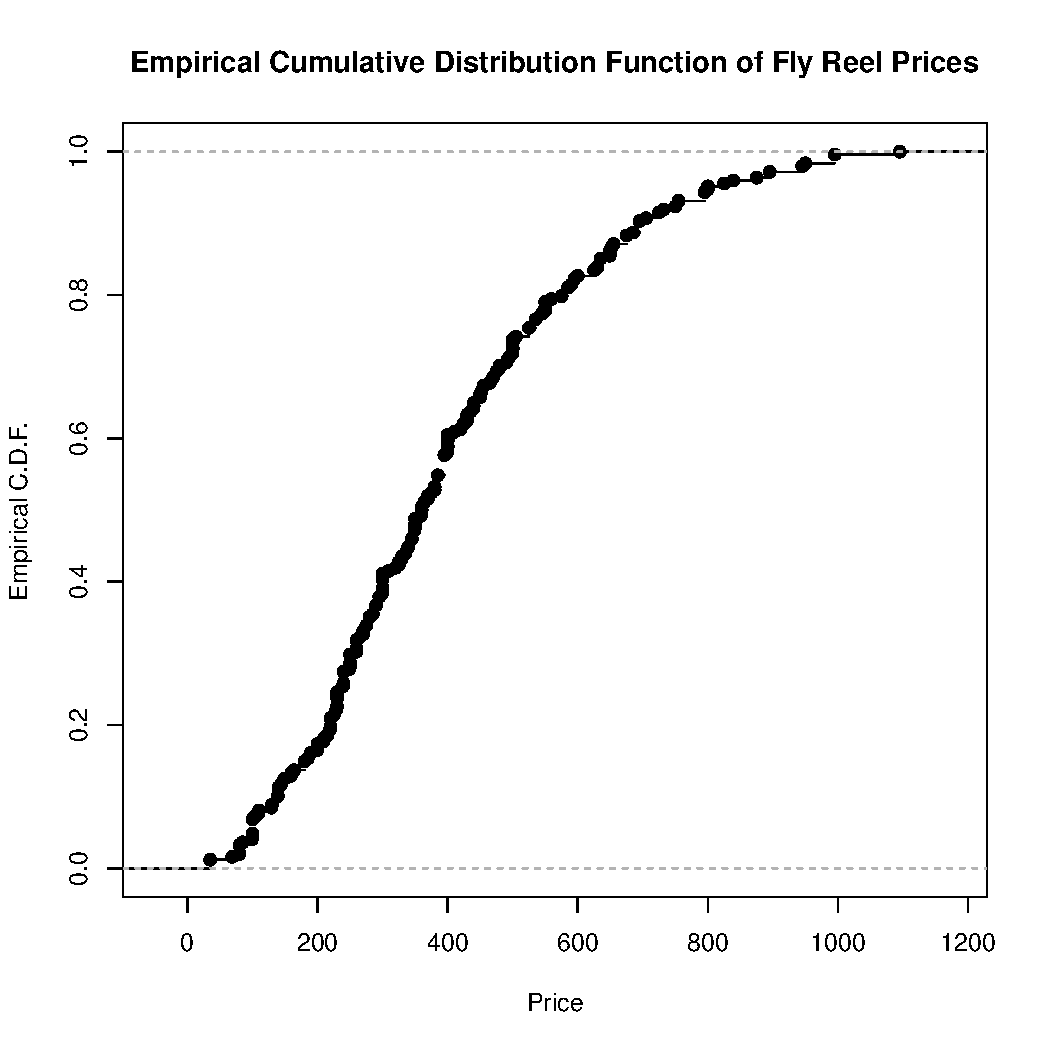
\includegraphics[scale = 0.5, keepaspectratio=true]{../Figures/ecdf_prices}
  \caption{Empirical Distribution Function of Fly Reel Prices} \label{fig:ecdf_prices}
\end{figure}


\section*{Relative Histogram of Fly Reel Prices}

Figure \ref{fig:hist_prices} is 
a histogram of fly reel prices. 

\begin{figure}[h!]
  \centering
  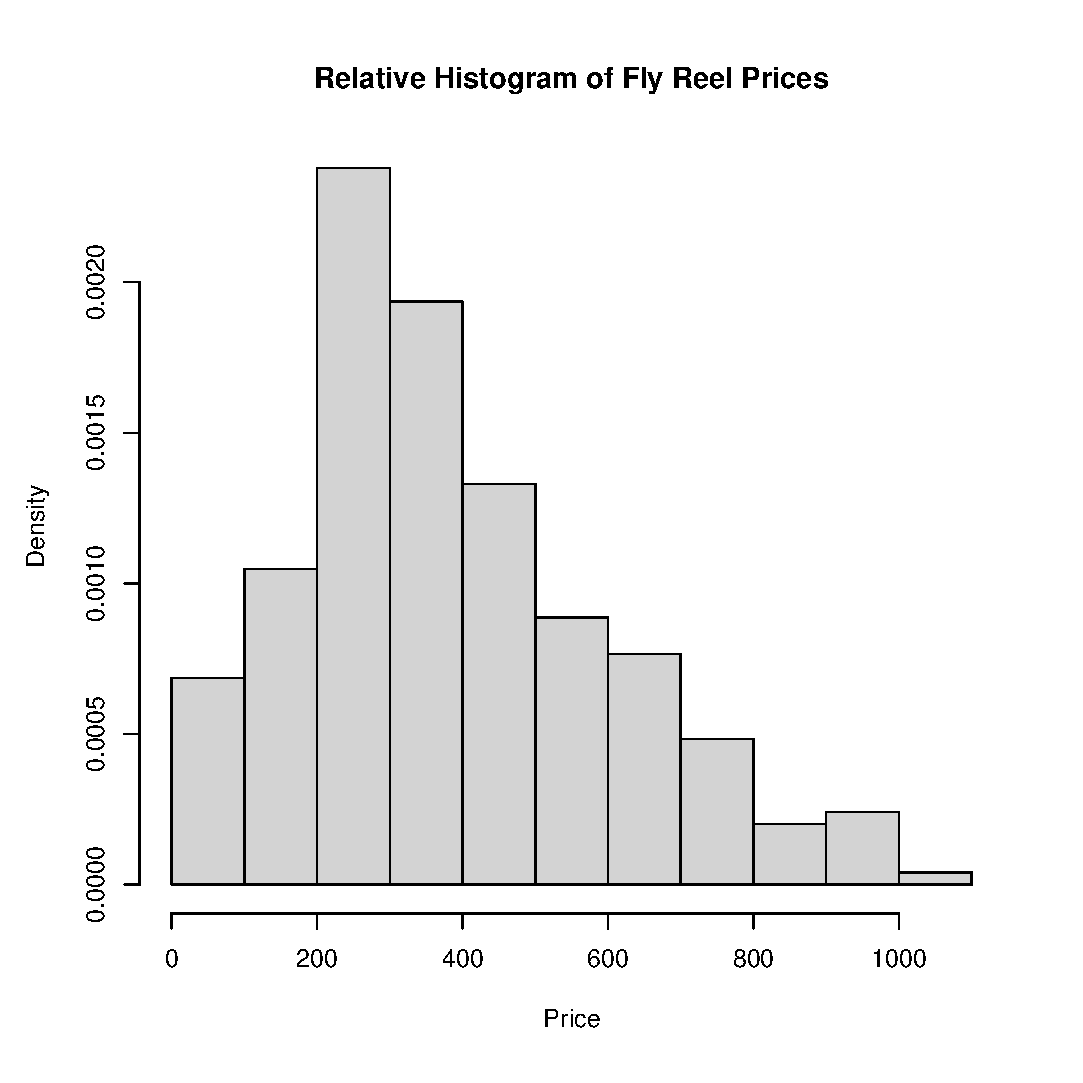
\includegraphics[scale = 0.5, keepaspectratio=true]{../Figures/hist_prices}
  \caption{Relative Histogram of Fly Reel Prices} \label{fig:hist_prices}
\end{figure}


\pagebreak
\section*{Probability Density Function of Fly Reel Prices}

Figure \ref{fig:density_prices} depicts 
the kernel-smoothed probability density function of the natural logarithm of
price.

\begin{figure}[h!]
  \centering
  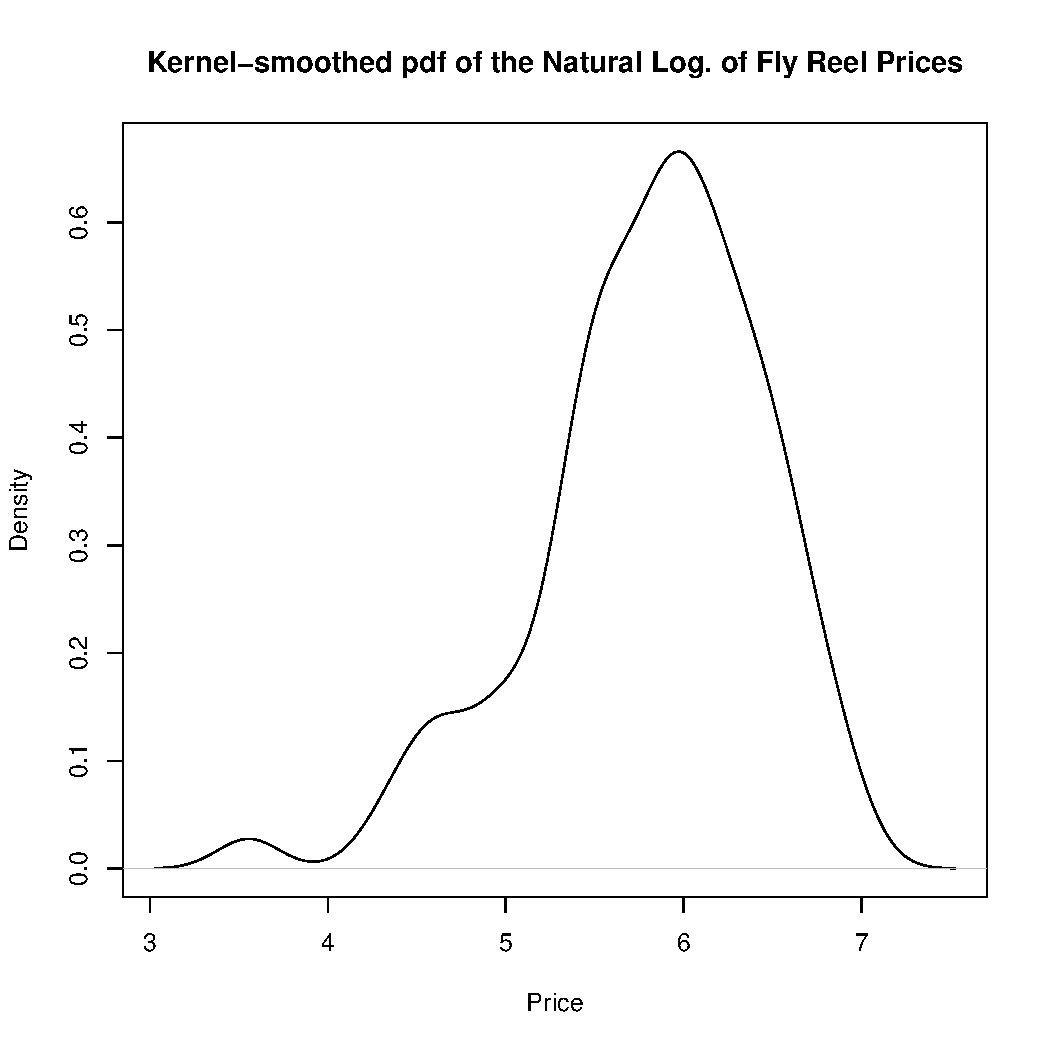
\includegraphics[scale = 0.5, keepaspectratio=true]{../Figures/density_prices}
  \caption{Probability Density Function of Fly Reel Prices} \label{fig:density_prices}
\end{figure}






\clearpage
\pagebreak
\subsection{Probability Density Function By Country of Manufacture}

Now we investigate the prices of fly reels made in the USA
compared to those made in China and Korea.
Figure \ref{fig:dens_by_country} shows the 
kernel density estimate of the prices of 
fly reels made in the USA in blue,
those made in China in red, 
and those made in Korea in green.
% 
The modes of the distributions are similar, 
however, we observe more variability in the prices of fly reels
made in Korea. 
The distribution of fly reels made in the USA is shifted 
toward the higher price range, compared to those made in other countries.
This indicates mild support for a ``Made in America'' premium
but we should also consider that it may be explained by 
the features of the reels made in the USA. 
We will investigate this further in regression analysis 
and other modeling approaches. 


\begin{figure}[h!]
  \centering
  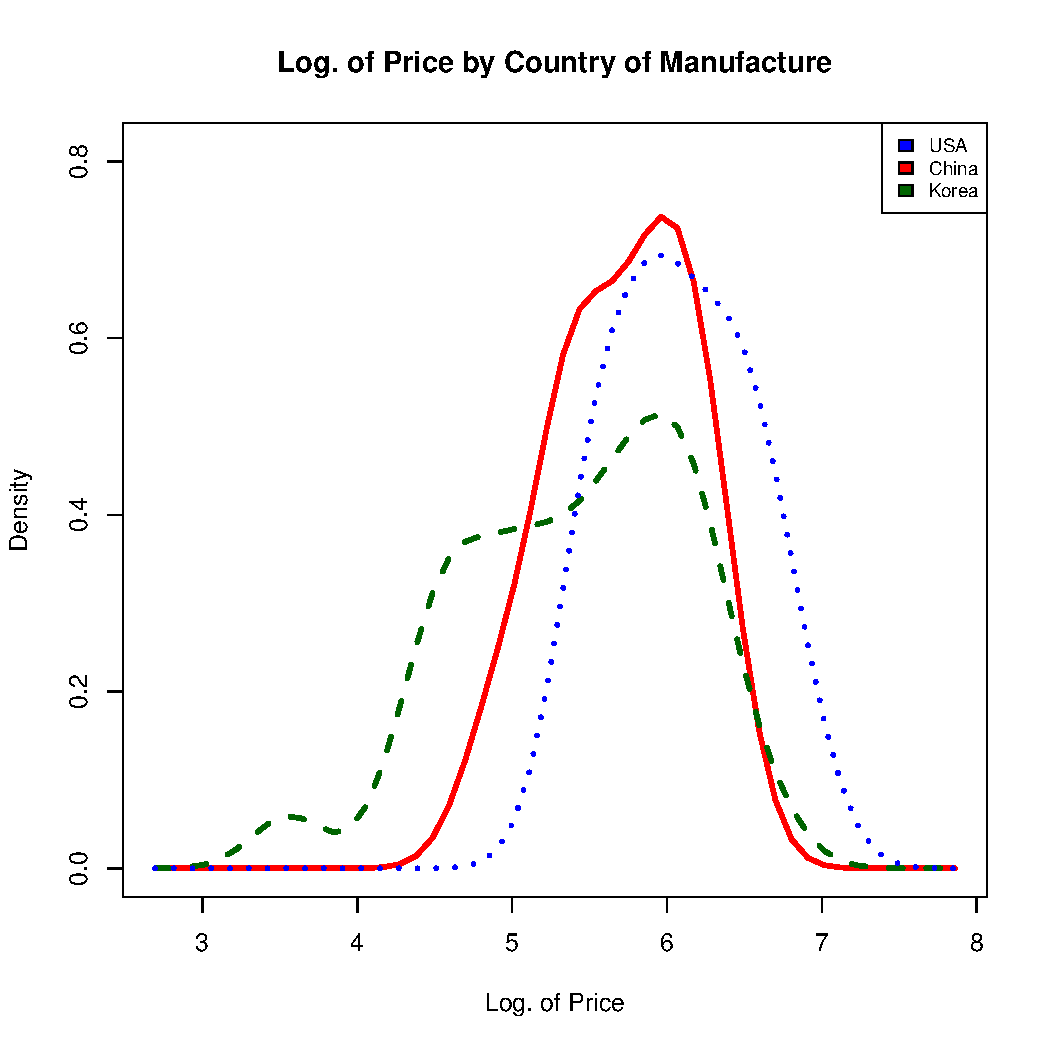
\includegraphics[scale = 0.5, keepaspectratio=true]{../Figures/dens_by_country}
  \caption{Densities of Log. Fly Reel Prices by Country of Manufacture} \label{fig:dens_by_country}
\end{figure}




%%%%%%%%%%%%%%%%%%%%%%%%%%%%%%%%%%%%%%%%
\end{document}
%%%%%%%%%%%%%%%%%%%%%%%%%%%%%%%%%%%%%%%%
